\chapter{Resultados}
\label{chap:resultados}

A seguir são apresentados os resultados do estudo conduzido para cada um dos motores de jogo, aplicando as recomendações mencionadas na documentação de cada um e utilizando o cenário base de testes. Como cada motor utiliza o seu próprio formato de arquivo para manipular os \textit{assets}, para que fosse possível replicar o mesmo cenário nos três motores foi necessário utilizar um cenário pré-modelado, onde os objetos 3D foram posicionados fixamente.

A cena de testes consiste em várias cópias de um conjunto de objetos, dentre eles uma casa, algumas pedras, uma malha que representa a água, um plano para o chão, algumas árvores e cogumelos como mostrado na Figura \ref{fig:cena}. Esses objetos foram duplicados até que fosse obtido um valor médio de taxa de quadros dentro do padrão aceitável para jogos eletrônicos de 30 FPS.

\begin{figure}[h!]
    \centering
    \Caption{\label{fig:cena} Cena padrão de testes}	
    \UNIFORfig{}{
        \fbox{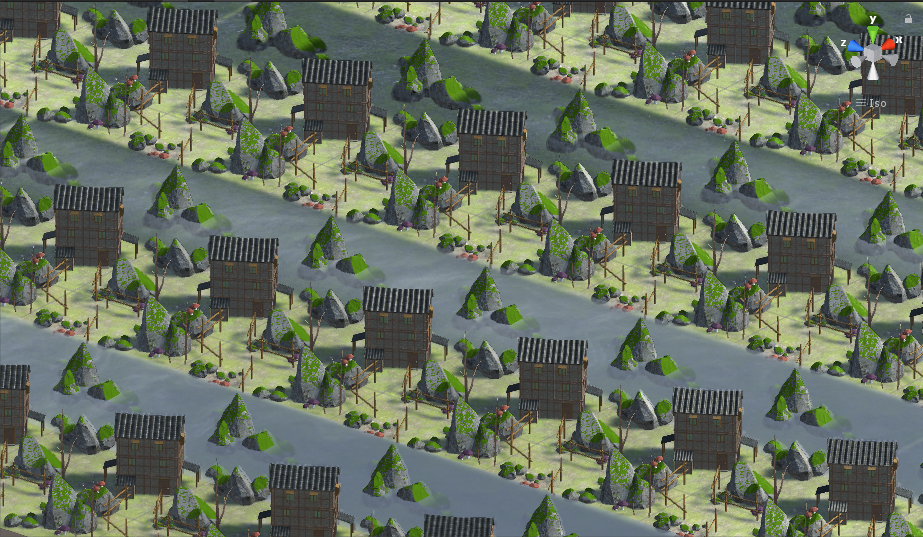
\includegraphics[width=10cm]{figuras/figura-cena}}
    }{
        \Fonte{Elaborado pelo Autor (2021)}
    }	
\end{figure}

\section{Discussão dos resultados na Godot}
\label{sec:resultado-godot}

A cena de teste foi replicada na Godot engine preservando as caracterísiticas fundamentais de número de triângulos (vértices) e materiais (shaders). Obviamente, houve necessidade de adaptação nos shaders de musgo sobre rochas e no shader de água devido ao fato do motor de renderização da engine fazer uso de GLSL.

Aqui é interessante destacar que a Godot executa automaticamente o culling para evitar a renderização de objetos que estão fora da janela de exibição. Isso funciona bem para jogos que acontecem em uma pequena área, no entanto, isso pode rapidamente se tornar problemático para níveis maiores.

Seguindo a recomendação da documentação da Godot, foi utilizado o cozimento de iluminação. Os mapas de luz cozidos são um fluxo de trabalho alternativo para adicionar iluminação indireta a uma cena. 

Lightmaps preparados funcionam bem em PCs de baixo custo e dispositivos móveis, visto que eles quase não consomem recursos em tempo de execução. Os mapas de luz preparados podem ser usados opcionalmente para armazenar iluminação direta, o que fornece ainda mais ganhos de desempenho (LINIETSKY; MANZUR, 2021)\nocite{manzur2021}.

A iluminação de objetos é uma das operações de renderização mais caras. Iluminação em tempo real, sombras (especialmente luzes múltiplas) e GI são especialmente caros. Eles podem damandar muito de dispositivos móveis de baixa potência. O uso de iluminação cozida tem a desvantagem de não ser dinâmico. Em geral, se várias luzes precisam afetar uma cena, é melhor usar mapas de luz cozidos. O cozimento também pode melhorar a qualidade da cena, adicionando reflexos indiretos de luz (LINIETSKY; MANZUR, 2021).

A próxima etapa consistiu em desativar o filtro das texturas. Ler texturas é uma operação cara, especialmente ao ler várias texturas em um sombreador de fragmento. Além disso, a filtragem pode desacelerar ainda mais esse processso (filtragem trilinear entre mipmaps e cálculo da média). Ler texturas também é caro em termos de uso de energia, o que é um grande problema em celulares.

A Tabela \ref{qua:godot} mostra os resultados obtidos para a aplicação de cada etapa de otmização.

\begin{table}[h!]
	\Caption{\label{qua:godot} Dados de \textit{profiling} de renderização da Godot}\UNIFORqua{}{
	\begin{tabular}{|l|c|c|c|c|} \hline
		                         & FPS   & \makecell{Chamadas \\ de desenho} & \makecell{Vértices \\ desenhados} & \makecell{Uso de memória \\ de vídeo} \\ \hline
		Configuração padrão      & 24    & 26143               & 11079162            & 338.7 MB                \\ \hline
		Etapa 1                  &       &                     &                     &                         \\ \hline
		~Uso de luz cozida (Low) & 26    & 26143               & 11079162            & 446.7 MB                \\ \hline
		~Uso de luz cozida (Medium) & 24 & 26143               & 11079162            & 446.7 MB                \\ \hline
		~Uso de luz cozida (High) & 25   & 26143               & 11079162            & 446.7 MB                \\ \hline
		Etapa 2                  &       &                     &                     &                         \\ \hline
		~Filtro desativado & 19    & 36437               & 15995958            & 338.7 MB                \\ \hline
		~Filtro desativado (Sem sombras) & 28 & 26143 & 11079162 & 338.7 MB \\ \hline
	\end{tabular} 
	}{
		\Fonte{Elaborado pelo Autor (2021)}}
\end{table} 

A partir dos dados obtidos fica nítido que o cozimento de luzes não se mostrou como uma solução efetiva para melhoria de performance, pois não aumentou de maneira considerável a taxa de quadros por segundo. 

Também foi possível notar que o uso de memória aumentou, o que já era esperado tendo em vista que o cozimento de luzes processa as sombras em um arquivo de textura que é salvo em memória para ser lido em tempo de execução. 

A etapa mais efetiva para ganho de desempenho acabou sendo o desativamento das sombras, com isso foi possível chegar mais próximo do objetivo de 30 FPS. Por último, desativar o filtro não se mostrou como uma medida viável visto que prejudicou a performance.

\section{Discussão dos resultados na Unreal}
\label{sec:resultado-unreal}

Na Unreal, um ponto positivo vai para a existência de materiais de ambiente (Grama, tijolos, pedras e até água) já prontos para serem utilizados, e inclusive com otimizações de performance como nível de detalhe e tesselação, dentro da pasta de conteúdo inicial do template de projeto padrão. Isso ajuda a reduzir bastante o trabalho dos desenvolvedores ao implementar shaders em seus jogos.

A primeira recomendação na documentação da Unreal sugere desativar a projeção de sombra, que é uma opção que vem habilitada por padrão. As sombras fazem com que os objetos pareçam estar ancorados no mundo e dão ao observador uma sensação de profundidade e espaço. 

Sombras estáticas não são custosas no que diz respeito à renderização, mas sombras dinâmicas podem ser um dos maiores problemas de desempenho. Em média, as luzes de projeção de sombras dinâmicas móveis são as mais custosas (EPIC GAMES, 2021).

Para a realização desta etapa, foi desativa a projeção de sombra individualmente para cada malha e em seguida, com a projeção das malhas reativada, foi desativado apenas na fonte de luz direcional.

Por padrão, o Unreal Engine usa um renderizador diferido, pois ele fornece maior versatilidade e concede acesso a mais recursos de renderização. A renderização diferida não é apenas mais rápida, mas também oferece melhores opções de anti-aliasing, o que gera melhores aspectos visuais.

A renderização direta fornece uma linha de base com passagens de renderização mais rápidas. A segunda etapa então consistiu em mudar, nas configurações do projeto, o modo de renderização de diferido para direto.

A próxima etapa consistiu em ajustar a oclusão de HZB (\acrlong{HZB}) que tem um custo constante alto, mas um custo por objeto menor. A oclusão HZB funciona da mesma forma que a oclusão padrão, exceto que é mais conservadora na maneira que seleciona objetos, o que significa que menos objetos são eliminados como resultado (EPIC GAMES, 2021). 

Ele usa uma versão \textit{mipmap} do alvo de renderização de profundidade de cena para verificar os limites de um ator. Também requer menos buscas de textura ao amostrar de um \textit{mipmap} menos detalhado (EPIC GAMES, 2021)\nocite{unrealdocs}.

A Tabela \ref{qua:unreal} mostra os resultados obtidos para a aplicação de cada etapa de otmização.

\begin{table}[h!]
	\Caption{\label{qua:unreal} Contagem de elementos presentes na cena de teste}\UNIFORqua{}{
	\begin{tabular}{|l|c|c|c|} \hline
		            & Vértices  & Triângulos & Qtd.  \\ \hline
		Casa        & 6901      & 4264       & 72    \\ \hline
		Plano       & 4         & 2          & 144   \\ \hline
		Árvores     & 794       & 368        & 288   \\ \hline
		Cercas      & 7156      & 3632       & 360   \\ \hline
		Cogumelos   & 2208      & 1056       & 360   \\ \hline
		Rochas      & ---       & ---        & ---   \\ \hline
		~Tipo 1     & 576       & 338        & 432   \\ \hline
		~Tipo 2     & 554       & 338        & 144   \\ \hline
		~Tipo 3     & 690       & 426        & 288   \\ \hline
		~Tipo 4     & 512       & 280        & 216   \\ \hline  
		~Tipo 5     & 120       & 62         & 72    \\ \hline
		Água        & 8         & 12         & 4     \\ \hline
		Soma        & 19523     & 10778      & 2380 \\ \hline
		Total       & 46464740  & 25651640   & ---   \\ \hline
	\end{tabular} 
	}{
		\Fonte{Elaborado pelo Autor (2021)}
	}
\end{table} 

A análise dos dados obtidos permitiu concluir que a melhor performance de taxa de quadros por segundo (39.67 FPS) ocorreu utilizando o modo de renderização direto com resolução de 75\%. Apesar de que esse modo adicionou aproximadamente 7 ms de tempo extra de renderização. Em compensação o uso máximo de mémoria foi reduzido em cerca de 12\%.

Além disso o modo direto permitiu que a Unreal fosse capaz de renderizar mais triângulos (e consequentemente realizar mais chamadas de desenho) sem que houvesse uma perda extrema de performance.

A aplicação de técnicas de otimização de performance na Unreal se mostra mais difícil por exigir um conhecimento da ferramenta de console da engine para aplicar comandos necessários para alterar aspectos que afetam a performance.

Um detalhe importante para levar em consideração é que ao invés de fornecer alternativas embutidas na própria engine, ela recomenda e oferece soluções de terceiros para realizar benchmark e otimizações de gráficos. Além disso, a sua documentação, diferente da Unity, não aborda tantas opções de melhorias de performance em um clique. 

Por isso ela é considerada um motor de jogo mais apropriado para usuários avançados, por entender que esses já possuem o conhecimento das técnicas necessárias para melhorar a performance e conseguem aplicá-las sem o auxilio de opções simples embutidas na engine.

Por fim, é importante salientar que desempenho é um tópico onipresente na criação de jogos em tempo real. Para criar a ilusão de imagens em movimento, uma taxa de quadros de pelo menos 15 quadros por segundo é necessária. Dependendo da plataforma e do jogo, 30, 60 ou até mais quadros por segundo podem ser o alvo (EPIC GAMES, 2021).

A Unreal Engine oferece muitos recursos e eles têm diferentes características de desempenho. A fim de otimizar o conteúdo ou código para atingir o desempenho necessário, é preciso ver onde o o desempenho é gasto. Cada caso é diferente e algum conhecimento sobre os componentes internos de hardware e software é necessário (EPIC GAMES, 2021). 


\section{Discussão dos resultados na Unity}
\label{sec:resultado-unity}

Na Unity foi criado um novo projeto com template 3D. Em seguida foram importados os modelos dos objetos para compor a cena. Ao importar os objetos foram removidas as importações de materiais e animações, pois estes não serão utilizados. A cena final é composta por uma câmera com posição fixa e contém aproximadamente 3 milhões e 300 mil triângulos (5 milhões e 500 mil vértices) resultando em 7211 \textit{batches} (chamadas de desenho).

Para a criação dos materiais, foram utilizados os padrões da engine que consistem no shader de superfície padrão, exceto para a implementação de um shader de musgo que afeta as pedras e para o shader de água. Ambos foram escritos utilizando a linguagem \textit{ShaderLab} e constam nos Anexos \ref{an:codigo-fonte-musgo-unity} e \ref{an:codigo-fonte-agua-unity} respectivamente.

Por padrão, a Unity importa um rig genérico para modelos de não personagens. Isso faz com que um componente Animator seja adicionado se o modelo for instanciado no tempo de execução. Se o modelo não for animado por meio do sistema de animação, isso adiciona sobrecarga desnecessária ao sistema de animação, porque todos os animadores ativos devem ser marcados uma vez por quadro (UNITY TECHNOLOGIES, 2021)\nocite{unityTech2021}.

Desativar o rig em modelos não animados para evitar esta adição automática de um componente Animator e possível adição inadvertida de animadores indesejados a uma cena é uma boa prática para objetos não animados e foi utilizada nessa cena (UNITY TECHNOLOGIES, 2021). 

É importante ressaltar que ao criar um material na Unity ele já possui um shader padrão embutido, facilitando bastante a implementação de shaders básicos (como cores ou texturas). Ou seja, para implementar shaders simples não é necessário realizar nenhum tipo de programação.

Foram utilizadas as configurações pré-definidas da Unity (tamanho máximo de 2048x2048, compressão normal e algoritmo de redimensionamento Mitchell) para importação das texturas que compõem os materiais. A única mudança realizada foi a remoção do filtro bilinear.

As etapas de otimização seguem as recomendações descritas na documentação da Unity para melhorias de performance. A cada etapa foram medidas as estatísticas fornecidas pela engine para comparar os procedimentos.

A primeira etapa de otimização seguindo a recomendação da documentação da Unity consiste em utilizar tamanhos menores de textura. Para aplicações mobile, 2048x2048 ou 1024x1024 é um tamanho suficiente de atlas de textura, e 512x512 é um tamanho suficiente para texturas individuais aplicadas em modelos 3D. Em contrapartida isso pode gerar uma perda de qualidade visual.

A próxima etapa de otimização consiste em desabilitar o sinalizador de leitura e gravação dos modelos 3D, pois ele é habilitado por padrão para todos os modelos importados. A Unity exige que este sinalizador seja habilitado se um projeto estiver modificando uma malha em tempo de execução via \textit{script}, ou se a malha for usada como base para um componente MeshCollider (o que não é o caso nessa cena padrão). Se o modelo não for usado em um MeshCollider e não for manipulado por scripts, é recomendado desativar este sinalizador para salvar metade da memória do modelo.

Se o formato de compressão da textura selecionado não é adequado para a plataforma de destino, o Unity descompacta a textura quando ela é carregada, consumindo tempo de CPU e uma quantidade excessiva de memória. Esse é um problema mais comum em dispositivos Android, que geralmente oferecem suporte a formatos de compactação de textura amplamente diferentes, dependendo do chipset.

Mais uma etapa de otimização consiste em usar a compressão de malha quando for possível.  Habilitar a compactação de malha reduz o número de bits usados para representar os números de ponto flutuante para diferentes canais de dados de um modelo. Isso pode levar a uma pequena perda de precisão e os efeitos dessa imprecisão devem ser verificados pelos artistas antes do uso em um projeto final. É possível usar três diferentes níveis de compressão (Low, Medium, High).

Outra etapa recomendada pela Unity é o uso da funcionalidade \textit{Graphics jobs}, uma opção que determina se serão utilizadas \textit{worker threads} (são \textit{threads} que performam uma única tarefa, como \textit{culling} ou \textit{mesh skinning}). Em plataformas onde essa funcionalidade está disponível, ela pode melhorar consideravelmente a performance.

Uma técnica interessante consiste em reduzir a distância de projeção da câmera usando a propriedade \textit{Far Clip Plane}. Esta propriedade é a distância além da qual os objetos não são mais renderizados pela câmera. Para disfarçar o fato de que objetos distantes não são mais visíveis, é possível usar a névoa. Após reduzir a distância de 1000 para 77 foi possível obter o dobro de taxa de quadros (60 FPS).

Caso a névoa seja um aspecto indesejado no jogo, uma alternativa na próxima etapa consiste em ativar a oclusão para desativar a renderização de objetos que estão ocultos por outros objetos. A seleção de oclusão do Unity não é adequada para todas as cenas, pode levar a sobrecarga de CPU adicional e pode ser complexa para configurar, mas pode melhorar muito o desempenho em algumas cenas.

Focando na próxima etapa, é possível fazer uso da instanciação de GPU para desenhar (ou renderizar) várias cópias da mesma malha de uma vez, usando um número menor de chamadas. Isso é útil para desenhar objetos como edifícios, árvores, grama ou outras coisas que aparecem repetidamente em uma cena.

Esse é um método útil para renderizar malhas idênticas e cada instância pode ter parâmetros diferentes (por exemplo, cor ou escala) para adicionar variação e reduzir a aparência de repetição. Isso pode ainda reduzir o número de chamadas de desenho e melhorar significativamente o desempenho de renderização (UNITY TECHNOLOGIES, 2021)\nocite{unity2Tech2021}.

Há ainda uma etapa de definição do nível de cascatas de sombra. Basicamente, quanto mais cascatas forem utilizadas, menos as sombras são afetadas pelo \textit{aliasing} de perspectiva. Aumentar o número aumenta a sobrecarga de renderização. No entanto, essa sobrecarga ainda é menor do que seria no caso de um mapa de alta resolução em toda a sombra.

Outro processo descrito consiste em utilizar os shaders móveis otimizados embutidos na Unity; deve-se experimentar usá-los e ver se isso melhora o desempenho sem afetar a aparência do jogo. Esses shaders foram projetados para uso em plataformas móveis, mas são adequados para qualquer projeto. É perfeitamente normal usar shaders "móveis" em plataformas não móveis para aumentar o desempenho se eles fornecerem a fidelidade visual necessária para o projeto.

Devido a alta disponibilidade de dados de \textit{profiling} ofereceidos pela Unity, os dados foram divididos em mais de uma tabela para melhor visualização. A Tabela \ref{qua:unity} mostra os resultados obtidos para a aplicação de cada etapa de otmização para as estatísticas gráficas.

\begin{table}[h!]
	\Caption{\label{qua:unity} Dados estatísticos de renderização da Unity}\UNIFORqua{}{
	\begin{tabular}{|l|c|c|c|} \hline
		            & \makecell{\textit{Thread} \\ de renderização}  & \makecell{\textit{Batches} \\ (Salvo)} & FPS  \\ \hline
		Etapa 1 & & & \\ \hline
		~Textura 1024x1024 & 29.6 ms & 7211 (15342) & 28.1 \\ \hline
		~Textura 512x512 & 28.4 ms & 7211 (15342) & 28.9 \\ \hline
		Etapa 2 & & & \\ \hline
		~Sem Leitura e Escrita (Malha) & 26.5 ms & 7226 (15327) & 30.1 \\ \hline
		~Compressão baixa (Malha) & 28.7 ms & 7215 (15338) & 28.1 \\ \hline
		~Compressão média (Malha) & 31.6 ms & 7213 (15340) & 25.9 \\ \hline
		~Compressão alta (Malha) & 28.7 ms & 7199 (15354) & 28.6 \\ \hline
		Etapa 3 & & & \\ \hline
		~Graphic Job ativado & 29.2 ms & 7199 (15354) & 28.9 \\ \hline
		Etapa 4 & & & \\ \hline
		~Névoa ativada & 15.8 ms & 3397 (6778) & 56.7 \\ \hline
		~Culling ativado & 27.2 ms & 7199 (15354) & 29.8 \\ \hline
		~Instanciação de GPU & 14.7 ms & 2228 (20325) & 32.3 \\ \hline
		Etapa 5 & & & \\ \hline
		~Cascata de sombra (0) & 13.2 ms & 2056 (17783) & 41.4 \\ \hline
		~Cascata de sombra (2) & 14.2 ms & 2141 (18913) & 39.3 \\ \hline
		Etapa 6 & & & \\ \hline
		~Shaders \textit{mobile} & 28.1 ms & 7015 (15538) & 28.6 \\ \hline
	\end{tabular} 
	}{
		\Fonte{Elaborado pelo Autor (2021)}
	}
\end{table} 

Após análise dos dados acima fica bem claro que o uso da névoa foi a medida mais efetiva para melhorar a performance, chegando a marca de 56.7 FPS e um dos menores tempos de \textit{thread} de renderização. Isso também se deve ao fato de que o número de \textit{Batches} acaba sendo reduzido.

\textit{Batching} é o nome do processo de criação de lotes --- grupos de objetos que são enviados como apenas um para a GPU. O Unity faz lotes estáticos e dinâmicos. Objetos estáticos que compartilham exatamente o mesmo material serão enviados como um único objeto (lote). Objetos dinâmicos que compartilham exatamente o mesmo material serão enviados como um único lote sob certas circunstâncias. Sem lote, cada objeto teria que ser enviado como seu próprio lote, criando uma grande sobrecarga de CPU.

Outro ponto importante foi a utilização do nível 0 de cascata de sombra que também diminuiu bastante o tempo de \textit{thread} de renderização.

Já a Tabela \ref{qua:unity2} contém os dados referentes à memória de renderização obtidos pelo \textit{profiler}. A ferramenta de \textit{profiling} dá informações detalhadas sobre o desempenho do jogo. Se o jogo apresentar baixa taxa de quadros ou alto uso de memória, essa ferramenta pode mostrar o que está causando esses problemas e ajudar a corrigi-los.

A janela do \textit{Profiler}, mostra diferentes aspectos do desempenho do jogo. Por exemplo, uso de memória, quanto tempo de CPU está sendo usado para diferentes tarefas e com que frequência os cálculos físicos estão sendo realizados. É possível usar esses dados para ajudar a encontrar a causa dos problemas de desempenho e medir a eficácia de tentativas de correçãO (UNITY TECHNOLOGIES, 2021).

É importante entender que há um pequeno custo de desempenho ao usar a janela do Profiler para registrar dados. Isso é comum a todas essas ferramentas; não é possível registrar e exibir dados detalhados como esses sem alguma sobrecarga. Embora seja improvável que isso faça uma diferença significativa na maneira como o jogo é executado (UNITY TECHNOLOGIES, 2021).

\begin{table}[h!]
	\Caption{\label{qua:unity2} Dados de \textit{profiling} de renderização da Unity}\UNIFORqua{}{
	\begin{tabular}{|l|c|c|c|} \hline
		            & \makecell{Uso de VRAM \\ (MB)} & \makecell{Uso de \\ texturas} & \makecell{Renderização \\ de texturas} \\ \hline
		Etapa 1 & & & \\ \hline
		~Textura 1024x1024 & 39.1 --- 62.3 & 22.1 MB & 33.6 MB \\ \hline
		~Textura 512x512 & 39.1 --- 48.8 & 8.6 MB & 33.6 MB \\ \hline
		Etapa 2 & & & \\ \hline
		~Sem Leitura e Escrita (Malha) & 52.5 --- 62.2 & 8.6 MB & 47.0 MB \\ \hline
		~Compressão baixa (Malha) & 49.3 --- 59 & 8.6 MB & 43.8 MB \\ \hline
		~Compressão média (Malha) & 62.2 --- 71.9 & 8.6 MB & 56.7 MB \\ \hline
		~Compressão alta (Malha) & 59 --- 68.7 & 8.6 MB & 53.5 MB \\ \hline
		Etapa 3 & & & \\ \hline
		~Graphic Job ativado & 51.7 --- 61.3 & 8.6 MB & 46.2 MB \\ \hline
		Etapa 4 & & & \\ \hline
		~Névoa ativada & 51.6 --- 61.3 & 8.6 MB & 46.1 MB \\ \hline
		~Culling ativado & 62.6 --- 72.3 & 8.6 MB & 57.1 MB \\ \hline
		~Instanciação de GPU & 62.7 --- 72.3 & 8.6 MB & 57.2 MB \\ \hline
		Etapa 5 & & & \\ \hline
		~Cascata de sombra (0) & 51.6 --- 61.3 & 8.6 MB & 46.1 MB \\ \hline
		~Cascata de sombra (2) & 47.6 --- 57.3 & 8.6 MB & 42.1 MB \\ \hline
		Etapa 6 & & & \\ \hline
		~Shaders \textit{mobile} & 55.1 --- 61 & 4.9 MB & 49.6 MB \\ \hline
	\end{tabular} 
	}{
		\Fonte{Elaborado pelo Autor (2021)}
	}
\end{table} 

Aqui é possível perceber que em termos de uso de memória, a redução da resolução das texturas ajudou a diminuir 60\% da carga de uso. Por outro lado, a porção de memória destinada a renderização apenas aumentou.

Notou-se também que o melhor intervalo de uso de VRAM (\acrlong{VRAM}) ocorreu ao usar a menor resolução de textura (a baixa compressão de malha também gerou resultados interessantes). O uso dos shaders otimizados para dispositivos móveis embutidos na Unity ajudou a diminuir 3,7 MB de carga de uso de memória. O que no final das contas não fez uma diferença considerável.
